\documentclass[a4paper]{article}
\usepackage[spanish]{babel}
\usepackage[utf8]{inputenc}
\usepackage{charter}   % tipografia
\usepackage{graphicx}
%\usepackage{makeidx}
\usepackage{paralist} %itemize inline
\usepackage[colorinlistoftodos,prependcaption]{todonotes}
%\usepackage{float}
%\usepackage{amsmath, amsthm, amssymb}
%\usepackage{amsfonts}
%\usepackage{sectsty}
%\usepackage{charter}
%\usepackage{wrapfig}
%\usepackage{listings}
%\lstset{language=C}


\usepackage{color} % para snipets de codigo coloreados
\usepackage{fancybox}  % para el sbox de los snipets de codigo

\definecolor{litegrey}{gray}{0.94}

% \newenvironment{sidebar}{%
% 	\begin{Sbox}\begin{minipage}{.85\textwidth}}%
% 	{\end{minipage}\end{Sbox}%
% 		\begin{center}\setlength{\fboxsep}{6pt}%
% 		\shadowbox{\TheSbox}\end{center}}
% \newenvironment{warning}{%
% 	\begin{Sbox}\begin{minipage}{.85\textwidth}\sffamily\lite\small\RaggedRight}%
% 	{\end{minipage}\end{Sbox}%
% 		\begin{center}\setlength{\fboxsep}{6pt}%
% 		\colorbox{litegrey}{\TheSbox}\end{center}}

\newenvironment{codesnippet}{%
	\begin{Sbox}\begin{minipage}{\textwidth}\sffamily\small}%
	{\end{minipage}\end{Sbox}%
		\begin{center}%
		\vspace{-0.4cm}\colorbox{litegrey}{\TheSbox}\end{center}\vspace{0.3cm}}



\usepackage{fancyhdr}
\pagestyle{fancy}

%\renewcommand{\chaptermark}[1]{\markboth{#1}{}}
\renewcommand{\sectionmark}[1]{\markright{\thesection\ - #1}}

\fancyhf{}

\fancyhead[LO]{Sección \rightmark} % \thesection\ 
\fancyfoot[LO]{\small{Aldasoro, Chamo, Galli, Noriega, Previgliano \& Zimenspitz}}
\fancyfoot[RO]{\thepage}
\renewcommand{\headrulewidth}{0.5pt}
\renewcommand{\footrulewidth}{0.5pt}
\setlength{\hoffset}{-0.8in}
\setlength{\textwidth}{16cm}
%\setlength{\hoffset}{-1.1cm}
%\setlength{\textwidth}{16cm}
\setlength{\headsep}{0.5cm}
\setlength{\textheight}{25cm}
\setlength{\voffset}{-0.7in}
\setlength{\headwidth}{\textwidth}
\setlength{\headheight}{13.1pt}

\renewcommand{\baselinestretch}{1.1}  % line spacing


% \setcounter{secnumdepth}{2}
\usepackage{underscore}
\usepackage{caratula}
\usepackage{url}


% ******************************************************** %
%              TEMPLATE DE INFORME ORGA2 v0.1              %
% ******************************************************** %
% ******************************************************** %
%                                                          %
% ALGUNOS PAQUETES REQUERIDOS (EN UBUNTU):                 %
% ========================================
%                                                          %
% texlive-latex-base                                       %
% texlive-latex-recommended                                %
% texlive-fonts-recommended                                %
% texlive-latex-extra?                                     %
% texlive-lang-spanish (en ubuntu 13.10)                   %
% ******************************************************** %



\begin{document}


\thispagestyle{empty}
\materia{Ingenier\'ia de Software I}
\submateria{Segundo Cuatrimestre de 2015}
\titulo{Trabajo Práctico II}
\subtitulo{Fecha de entrega: 5 de Noviembre}
\integrante{Aldasoro Agustina}{86/13}{agusaldasoro@gmail.com}
\integrante{Chamo Nicolás}{282/13}{nicochamo@hotmail.com}
\integrante{Galli Cristian}{538/11}{lococris88@hotmail.com}
\integrante{Noriega Francisco}{660/12}{frannoriega.92@gmail.com}
\integrante{Previgliano Fabricio}{430/13}{fjprevi@gmail.com}
\integrante{Zimenspitz Ezequiel}{155/13}{ezeqzim@gmail.com}

\maketitle
\newpage

\thispagestyle{empty}
\vfill


\thispagestyle{empty}
\vspace{3cm}
\tableofcontents
\newpage


%\normalsize\newpage

\section{Introducci\'on}

En el presente trabajo se aborda la tem\'atica del \emph{proceso electoral}. El cual dividimos en tres etapas: \textit{Preparaci\'on, Sufragio y Conteo}.\\


\subsection{Preparación}

En la etapa de preparación, el Ministerio provee un listado con los datos personales de todo el padrón, y lo carga en el sistema, permitiendo así la exposición de los datos a través de la interfaz web. De esta manera, un elector podrá consultar el padrón, y de no figurar en él, se dirigirá al ministerio, donde el sistema le permitirá al ministerio ingresar nuevos votantes  (hasta determinada fecha límite) asignándoles una mesa válida. 

A su vez, electores, fiscales generales y partidos políticos, podrán revisar el código fuente, el cual fue subido a la interfaz web, para ver que no haya ninguna irregularidad en el mismo.\\

Pasada dicha fecha, el ministerio suministra la información sobre las escuelas disponibles para votar al sistema, y procede a activar la opción “Asignar escuela y mesa” a cada elector, donde el sistema realiza dicha asignación automáticamente. A su vez, asigna de manera aleatoria los presidentes de mesas, ponderando a los que nunca lo fueron previamente.\\

Dado que el ministerio precisa conocer a los presidentes de mesa designados, el sistema permite consultar quienes son los mismos, de manera que el Ministerio pueda comunicarse con ellos. En caso de que algún notificado no pudiera estar presente (con justificación válida), el sistema permitirá al Ministerio elegir uno nuevo. Quedará a cargo del Ministerio, la capacitación de los mismos.\\

Posteriormente, los partidos políticos presentan sus candidatos al Ministerio (hasta determinada fecha límite). Pasada la misma, el Ministerio carga esta información en la versión Web para que esté disponible a consultar y el equipo técnico del mismo graba la información en las máquinas impresoras de voto. En este momento, también, asigna una máquina impresora de voto a cada mesa, más dos extra por escuela (en caso de que suceda algún exabrupto), sumado a una máquina extra (que sólo será utilizada para el envío del conteo de votos) y un cable de conexión de teléfono. Cada máquina posee una batería que dura 3 hs sin estar conectada a alimentación eléctrica. 

El sistema proveerá una contraseña única para todas las máquinas, la cual permite acceder al “Modo envío”, y adem\'as una contraseña única por cada Fiscal General de escuela, quienes ser\'an utilizadas en el momento de cargar los resultados de la elección, lo que permitir\'a el env\'io de datos encriptados mediante RSA.\\

Luego, se prepara un lote de boletas para cada mesa, considerando entre ellas a la boleta donde se imprimirán los resultados. Por cada mesa, se asignan además una cantidad extra de boletas, en caso de que algún votante termine utilizando más de una (dado que se puede arrepentir antes de efectuar su voto). Las boletas tienen dos troqueles iguales, los cuales permiten identificar que la misma no fue intercambiada por el votante al momento de realizar la elección, evitando así este tipo de fraude. Las mismas tienen un espacio para impresión con tinta, y un chip grabable dentro.\\

Después, el Ministerio imprime copias del padrón correspondiente a cada mesa, para que sean utilizados por los presidentes de mesa, fiscales y las escuelas, estas mismas lo deberán dejar en un lugar visible para que los votantes puedan consultarlo. También prepara las urnas, armando tantas como cantidad de mesas haya, las cuales poseen una identificación de la mesa a la que pertenecen; y provee auriculares para cada escuela, que recibirán los encargados de las mismas, los cuales brindarán a los votantes no videntes una ayuda a la hora del sufragio. 

Es el ministerio también el encargado de entregarle a cada Fiscal General las dos contraseñas, y un pendrive. La funcionalidad de este \'ultimo consistir\'a en que el fiscal lo inserte dentro de la m\'aquina de sufragio; luego el software dentro de \'el calcula el hash del programa dentro de la m\'aquina e informa si coincide con el hash original, el cual tiene almacenado.

Estando todo preparado, el Ministerio notifica a las fuerzas de seguridad qu\'e escuelas son las seleccionadas para la elección donde deberán brindar aporte.\\

Llegado el dia de la elección, el correo lleva a cada escuela correspondiente, la cantidad de máquinas de voto asignadas junto a las máquinas extra, todas con sus baterías correspondientes. Además, lleva las boletas, las urnas, las copias del padrón y los auriculares. Todo esto es recibido por el encargado, quien se los otorgará a los presidente de mesa y fiscales. Una vez allí, el fiscal general junto a los presidentes de mesa que ya estén presentes y las fuerzas de seguridad, distribuyen una mesa por aula. A su vez, se posicionan las urnas, las boletas y las máquinas de votación en su lugar correspondiente. Los auriculares permanecerán en posesión del Fiscal General, quien será el encargado de otorgarlo de ser necesario.\\

Cada presidente de mesa se ubica en su mesa respectiva. Si llega un votante a una mesa, y esta no cuenta con un presidente de mesa, el fiscal general de la escuela lo nombrará como presidente de dicha mesa. Cada presidente de mesa da inicio a la votación. Lo hace al activar una opción en la máquina de votación. El presidente de mesa es quien emitirá su voto primero acorde a lo explicado posteriormente.

A partir de ese momento, cualquier votante habilitado que llegue a su mesa podrá emitir sufragio.\\


\subsection{Sufragio}


Llega un votante a la mesa. En caso de tener alguna discapacidad, tiene prioridad en la cola. 

Si el votante lo necesitase, podrá requerir ayuda y/o auriculares al presidente de mesa quien se deberá contactar con el Fiscal General con el fin de conseguir los auriculares. Para personas que posean problemas de movilidad, se les permitirá imprimir su voto en máquinas ubicadas en planta baja, mientras que el presidente de mesa les acercará la urna, para que pueda depositar su boleta al finalizar el sufragio. Sólo usará la máquina impresora de voto de la misma, mientras que es responsabilidad del presidente de mesa acercar la urna para que su voto sea contabilizado en la mesa que le corresponde por el padrón.

En el caso de que no posea una discapacidad, espera en la cola de votación de la mesa. 
En ambos casos, cuando es su turno, el votante le entrega su DNI al presidente de mesa. Este verifica su identidad al asegurarse que la persona que le entregó el DNI es la poseedora del mismo, que se encuentra en el padrón correspondiente a la mesa, y que no votó todavía. Los fiscales de mesa hacen lo mismo. Si hay algún problema, el presidente de mesa y/o los fiscales notifican al fiscal general de la escuela. El mismo decidirá si la persona está apta para emitir voto o no.\\

Si el votante pasa la verificación, el presidente de mesa procede a entregarle la boleta y le retiene el DNI. A la boleta entregada, le quita un troquel que posee el código identificatorio, dejándola con el otro código idéntico en la boleta.
Luego, el votante se acerca la máquina impresora de voto e inserta la boleta.\\

Entonces, el sistema de la máquina muestra por pantalla las opciones de votar: por categoría o votar lista completa. Para ambos casos, se presentan las opciones (se incluye también la de voto en blanco) en posiciones aleatorias en la pantalla.

El votante podrá entonces elegir entre las opciones y al finalizar, obtener la boleta con su voto impreso (tanto en el papel como en el chip). El votante puede verificar en la máquina que lo impreso en el chip sea correcto.\\

Luego, el votante quita el troquel restante a la boleta, se lo entrega al presidente de mesa y si coincide con el retirado previamente, puede pasar a depositar la boleta en la urna siempre y cuando no haya cantado cuál será su voto. Si el votante canta su voto, la boleta quedará anulada impidiéndole ingresarla en la urna. 

Si el votante se arrepiente, puede pedir otra boleta y repetir el proceso.
Finalmente, el presidente de mesa le hace firmar al votante el padrón, y le devuelve el DNI conjunto a la constancia de voto.\\

En el caso de que falle alguna máquina, se pueden reemplazar por las dos de repuesto que posee cada escuela las cuales estarán a cargo del fiscal general. Si en una escuela dejan de funcionar más de dos máquinas, se podrá compartir la maquina de sufragio entre mesas, pero cada boleta deberá ser depositada en la urna correspondiente.\\

El fiscal general puede, en todo momento, utilizar el pendrive suministrado por el Ministerio, para chequear que el código que se ejecuta en cada máquina, es el correcto (acorde a lo explicado en la secci\'on anterior).\\

Pasadas las 18hs, las fuerzas de seguridad cierran las puertas de las escuelas. Y una vez terminados los comicios, empieza el conteo.\\

\subsection{Conteo}


El presidente de mesa abre la urna y pone a la máquina impresora de voto en “Modo de conteo”, dando así comienzo al conteo de cada voto. \\

Dado el caso en que no haya nada impreso en una boleta, o haya algo escrito a mano, se impugna el voto.

Si la boleta no fue altera, se inserta en la m\'aquina impresora de voto. Cuando la máquina lee el chip, lleva la cuenta de los votos procesados. Al pasar la boleta por la máquina, figura en la pantalla el voto grabado. 

Es responsabilidad tanto del presidente de mesa, como de los fiscales, corroborar que por cada boleta, el voto que se muestre en pantalla (obtenido por el lector del chip) coincida con lo impreso en la misma.\\

En caso de que ocurra alguna irregularidad, el presidente de mesa y/o fiscales lo comunicarán al fiscal general de la escuela. Frente a esta irregularidad, el fiscal deber\'a ordenar que se recuenten todos los votos, o bien podrá anular la mesa (si lo considera necesario).\\

Al finalizar el conteo, el presidente de mesa insertará una boleta vacía en la máquina impresora de voto, la cual grabará en el chip los votos contabilizados de la mesa. Además imprimirá con tinta en la boleta la cantidad de votos para cada categoría y así obtener una manera de contrastar lo grabado con lo contabilizado.

Luego, el presidente de mesa llevará la boleta con el conteo al Fiscal general, quien será el encargado de cargarla en la máquina de impresión de votos con conexión telefónica destinada al envío de resultados. El mismo posee dos contraseñas; al ingresar la primera, la máquina impresora de votos le permitirá ingresar al “Modo envío”. Una vez cargadas todas las boletas, las envía por el enlace telefónico al centro de cómputos nacional, esto lo hace bajo la incriptaci\'on RSA. El presidente de mesa podrá acompañarlo en todo momento para ver que se contabilice lo correcto.\\

El fiscal general puede, en todo momento, utilizar el pendrive suministrado por el Ministerio, para chequear que el código que se ejecuta en cada máquina, es el correcto.\\

Posteriormente, el presidente de mesa inserta la boleta con el conteo impreso en la urna junto a todas las boletas contabilizadas de la mesa. El presidente sella la urna, el fiscal general la agrupa con las otras que hay en escuela, y brinda al correo todas las urnas de su escuela e identifica a las urnas que hayan sido impugnadas. Además, envía el padrón para poder identificar a quienes votaron. El correo se encarga de enviarlas al centro de cómputos nacional.\\

El Sistema del Centro de Cómputos sólo contabilizará resultados de mesas que hayan sido cargados con contraseñas de Fiscal General válidas y correspondientes a las mesas de las urnas recibidas.
El Centro de Cómputos nacional calcula los resultados provisorios de las elecciones (como si hay ballotage, o la cantidad de diputados mediante el método D’Hont) con la información recibida por el enlace telefónico.

A las 20hs el Centro de Cómputos nacional publica los resultados del conteo provisorio en su página web.\\

Finalmente, el correo llevará todas las urnas al centro de cómputos nacional donde se realizará el conteo definitivo (No es posible saber a priori cuándo ocurrirá esto).



\newpage
\section{Presunciones}
- Presunciones: acá deberían listar aquellas cuestiones que asumieron por encima del enunciado. Estas cuestiones pueden provenir de alguna consulta con docentes. También pueden provenir de alguna especulación o interpretación que el grupo hizo.
\newpage
\section{Vistas}

Pasaremos a ahora a presentar los distintos diagramas para continuar modelizando nuestro problema.

En una primera instancia presentaremos el diagrama de clases, si bien presentamos el diagrama no estará acompañado de sus predicados de OCL, estos se presentaran posteriormente en la vista de las distintas etapas. 
Como dijimos anteriormente, presentaremos nuestra solución dividiendola en 3 etapas: Preparación, sufragio y conteo. 

Contamos con 5 tipos de diagramas, analizemos un poco las ventajas y desventajas de cada uno antes de comenzar.

\paragraph{Diagrama de contexto} 

El diagrama de contexto es una de las piedras angulares de este trabajo, nos permite observar las interacciones entre agentes. A su vez, no tenemos orden de las acciones ni una relación temporal lo cual nos impide modelizar muchas situaciones.

\paragraph{Diagrama de clases y OCL}

El diagrama de clases nos presenta una visión general de lo que vamos a modelizar, a su vez nos define un poco más las relaciones entre las clases de nuestro sistema. Permite dar una panorama general de como se comportan las clase entre ellas y que se le atribuye a cada una. Al mismo tiempo, el diagrama no permite expresar todo, para esto usaremos OCL, un lenguaje que expande al diagrama y nos permite expresar más relaciones entre clases.

\paragraph{Diagrama de casos de uso}

Este diagrama nos permite describir la interacción entre el sistema y los distintos actores 
externos. Junto a la descripción de los casos de uso, construye un detalle importante para la 
construcción del sistema.

\paragraph{Diagrama de Actividad}

El diagrama de actividad pone un orden relativo en los casos de uso. Y los relaciona aún más con los actores.

\paragraph{Máquinas de estado finitas}

La máquina de estados permite la composición entre varios actores con el mismo comportamiento y a su vez nos permite dar un orden temporal de los eventos. 


Presentaremos primero el diagra de contexto y el diagrama de clases.

\subsection{Diagrama de Contexto}
\todo[inline]{Aca va el diagrama de contexto}


\subsection{Diagrama de Clases}
\todo[inline]{Aca va el diagrama de clases}

Ya presentados el diagrama de contexto y el de clases podemos pasar a analizar para cada una de las etapas presentadas en la introducción mediante los distintos diagramas ya presentados.

\subsection{Preparación}


\subsubsection{Diagrama de actividad}

\todo[inline]{PONER EN SU LUGAR LOS DIAGRAMAS DE ACTIVIDAD}
\begin{figure}[h!]
\centering
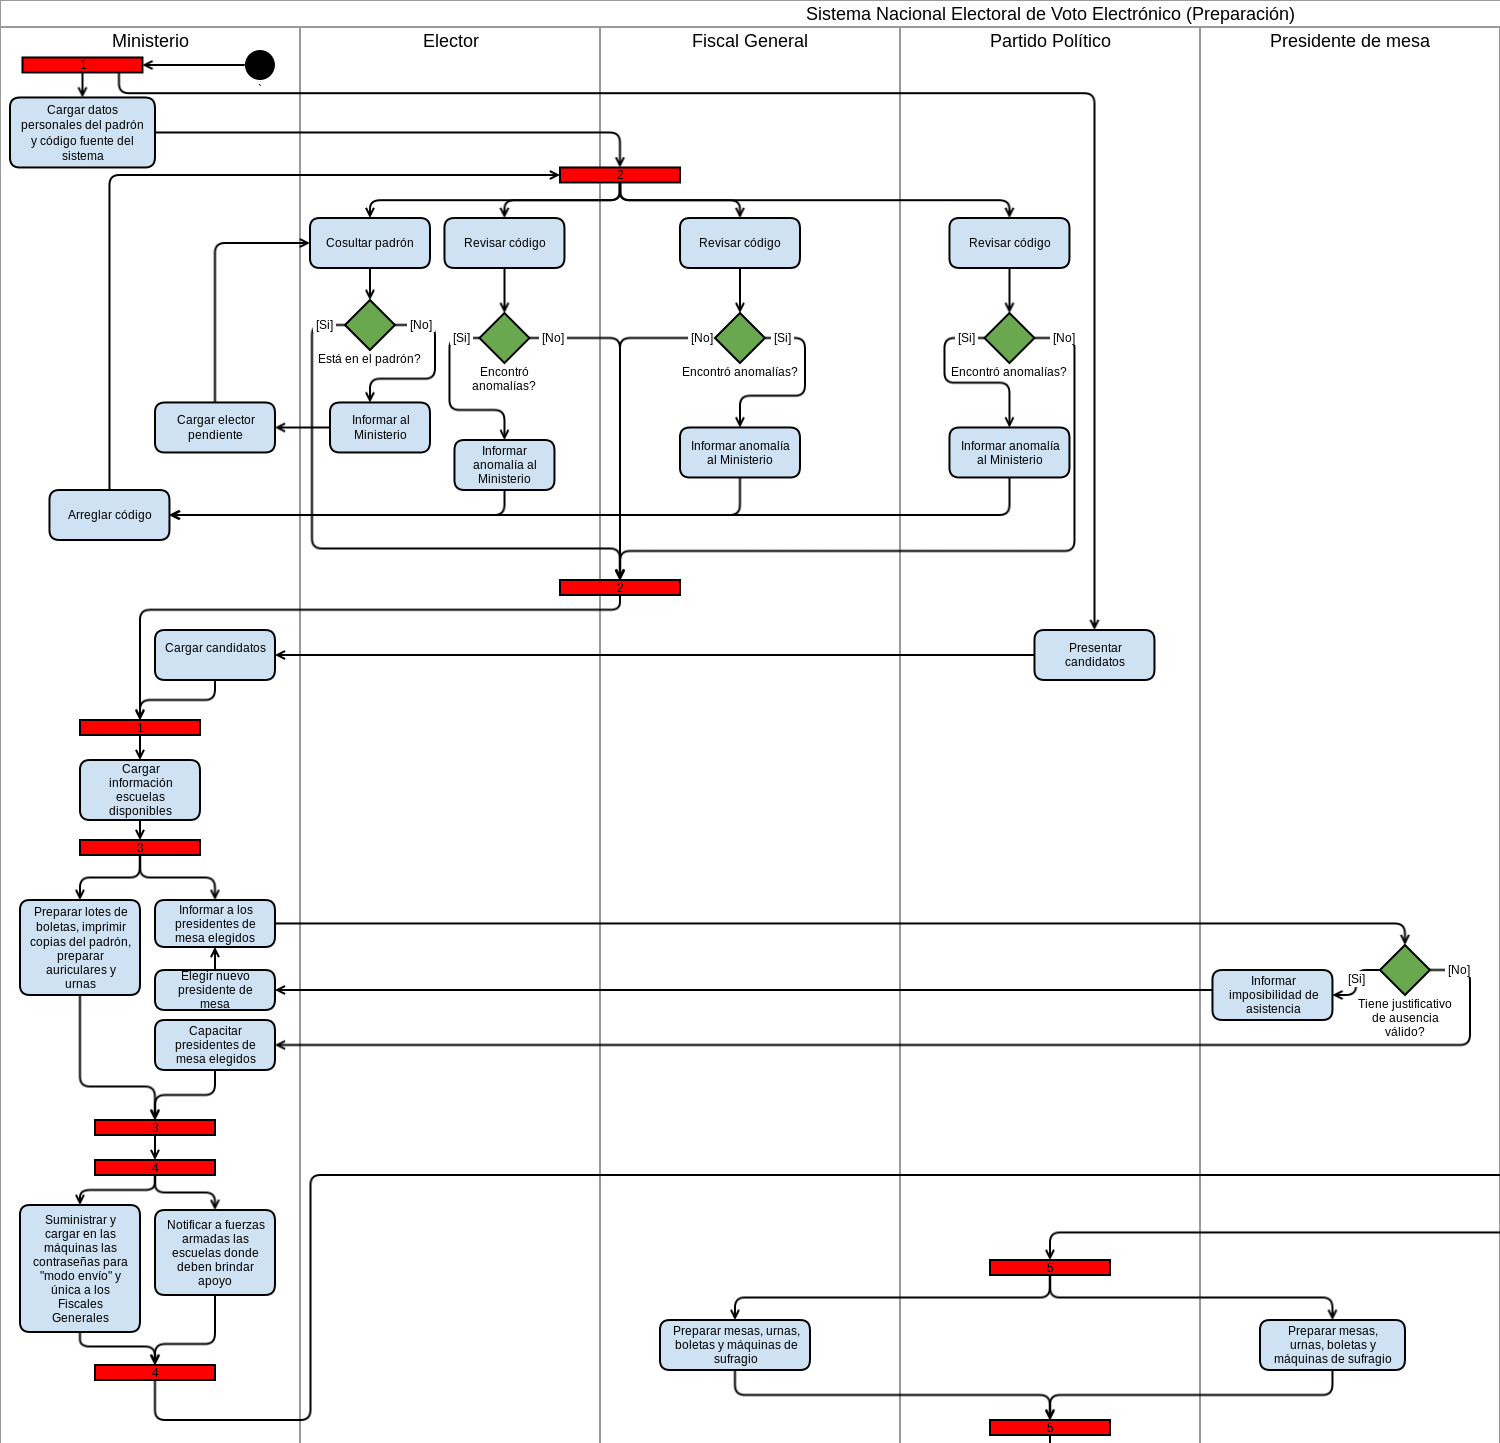
\includegraphics[scale=0.5]{imagenes/actividad/actividadPreparacion1}
%\captionof{figure}{Diagrama de actividad}
\end{figure}
<<<<<<< HEAD
\todo[inline]{Aca va el diagrama de actividad (ojo con la escala)}
=======

\begin{figure}[h!]
\centering
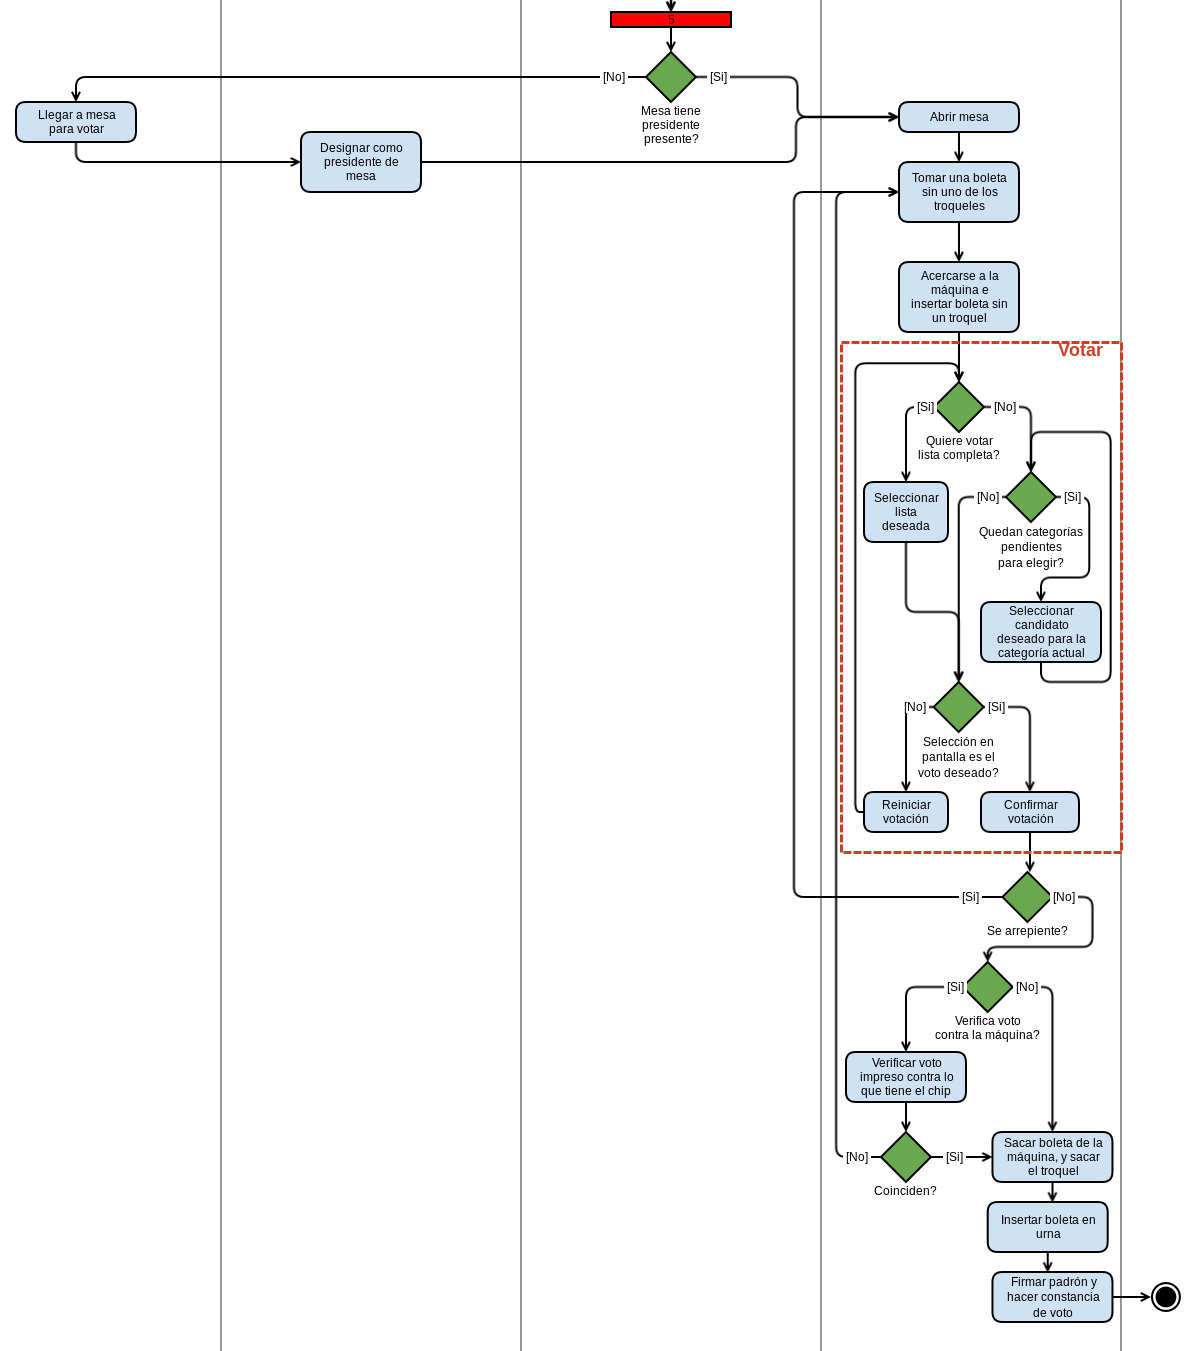
\includegraphics[scale=0.5]{imagenes/actividad/actividadPreparacion2}
\end{figure}

\begin{figure}[h!]
\centering
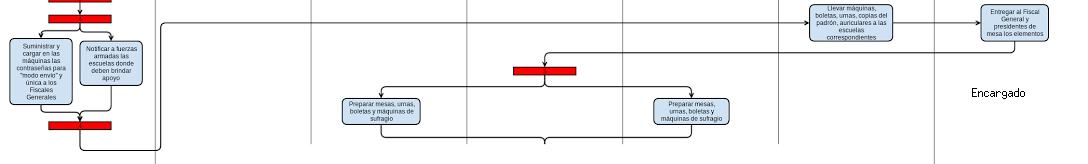
\includegraphics[scale=0.5]{imagenes/actividad/actividadPreparacion3}
\end{figure}
>>>>>>> ac9061ee9a2071afc042464a0c4c7ba3e049e030

\subsubsection{Máquina de estado finito}

Para esta sección fu necesario construir 2 máquinas de estado.

\begin{figure}[H]
\centering
%\includegraphics[scale=0.45]{}
%\captionof{figure}{Máquina de fechas limite}
\end{figure}

Esta máquina de estado nos define los tiempos de la etapa, es decir enmarca los tiempos de los casos de uso presentados anteriormente. Es importante notar que las transiciones marcadas en esta FSM corresponden a las acciones mostradas en el diagrama de actividad con el mismo nombre.

\begin{figure}[H]
\centering
%\includegraphics[scale=0.45]{}
%\captionof{figure}{Máquina de elección aleatoria de presidente de mesa}
\end{figure}



\subsubsection{Casos de uso}

Veamos primero el diagrama de casos de uso y luego veremos el detalle de los distintos casos de uso.

Es importante notar que el detalle de casos de uso, nos interioriza mucho en mucho de lo mencionado anteriormente en el diagrama de actividad. 

\todo[inline]{Acá va el diagrama de casos de uso}

Al ver el diagrama, se nota algo interesante. Muchos agentes distintos terminan teniendo los mismos casos de uso que el elector. Si bien anteriormente tuvimos que distinguirlos y fue importante hacerlo, por sus interacciones esternas al sistema, cuando interactuan con el sistema son lo mismo que un elector.

Nos muestra también la importancia del diagrama de contexto para identificar agentes que quizas no interactuen con el sistema pero son escenciales a la construcción del mis.

\textbf{Caso de Uso: Autenticandose}

\textbf{Actores:} Ministerio

\textbf{Pre:} -

\textbf{Post:} El ministerio se encuentra autenticado en el sistema web.
\begin{table}[h!]
	
 \begin{tabular}{|p{7.5cm} | p{7.5cm}|} 
 \hline
 \textbf{Curso normal} & \textbf{Curso Alternativo} \\
 \hline
 %\hline
 1. El ministerio ingresa al sistema web. & \\
 \hline
 
 2. El sistema le pide usuario y contraseña para ingresar. & \\
 \hline 
 3. El ministerio ingresa usuario y contraseña, y elige la opción “Ingresar”. & \\
 \hline 
 4. La información se valida, y se muestra el menú principal. & 
4.1. La información de inicio no es correcta, por lo que se muestra un mensaje de error. Ir al paso 2.
\\
 \hline 
 5. Fin de CU. & \\

 \hline
 \end{tabular}

\end{table}


\textbf{Caso de uso: Cargando padrón}
\textbf{Actor}: Ministerio
\textbf{Pre}: El ministerio se encuentra autenticado en el sistema, el padrón no fue cargado, y todavía no pasó la fecha límite para modificaciones al padrón.
\textbf{Post}: El padrón se encuentra cargado en el sistema y puede ser consultado desde la web.
\begin{table}[h!]
	
 \begin{tabular}{|p{7.5cm} | p{7.5cm}|} 
 \hline
 \textbf{Curso normal} & \textbf{Curso Alternativo} \\
 \hline
1. El ministerio importa el padrón suministrando un archivo con todos los datos de los ciudadanos capacitados para votar.
El archivo importado es de formato .csv, con las siguientes columnas: Nombres, Apellidos, DNI, Dirección, Ciudad, Provincia y Sexo. & \\
\hline

2. El sistema guarda los datos y los publica en la web, para que sean consultados. &
2.1. Si ocurre un error durante la importación, mostrar mensaje de error e ir al fin del caso de uso. \\
\hline
3. Fin de CU. & \\

 \end{tabular}

\end{table}





\textbf{Caso de Uso: Ingresando nuevo votante}

\textbf{Actores:} Ministerio

\textbf{Pre:} El ministerio se encuentra autenticado en el sistema, el padrón se encuentra cargado en el sistema, y puede ser consultado desde la web.

\textbf{Post:} El padrón se actualiza en el sistema, agregando al nuevo votante.
\begin{table}[h!]
	
 \begin{tabular}{|p{7.5cm} | p{7.5cm}|} 
 \hline
 \textbf{Curso normal} & \textbf{Curso Alternativo} \\
 \hline

1. El ministerio ingresa los datos del nuevo votante en un formulario. & \\
\hline

2. El ministerio elige la opción de “Cargar votantes”. & \\
\hline

3. Se actualizan los datos en el sistema. & 3.1. Si existe un error en la carga, se muestra un mensaje con el error. Ir al paso 2. \\
\hline
4. Fin de CU. & \\
 \hline
 \end{tabular}

\end{table}

\textbf{Caso de uso: Cargando información sobre escuelas}

\textbf{Actor:} Ministerio

\textbf{Pre:} El ministerio se encuentra autenticado en el sistema, y pasó la fecha establecida para la modificación del padrón.

\textbf{Post:} El sistema posee la información de los electores y sus mesas correspondientes, y además designó un presidente de mesa para cada una. Esta información se encuentra consultable en la web.


\begin{table}[h!]
	
 \begin{tabular}{|p{7.5cm} | p{7.5cm}|} 
 \hline
 \textbf{Curso normal} & \textbf{Curso Alternativo} \\
 \hline

1. El ministerio importa la información sobre las escuelas suministrando un archivo con todos los datos de las escuelas. El archivo importado es de formato .csv, con las siguientes columnas: Nombre, Dirección, Ciudad, Provincia y Cantidad de aulas. & \\
\hline

2. El sistema guarda los datos importados y asigna a los electores a las escuelas más cercanas, asignando una mesa a cada uno. &
2.1. Si ocurre un error durante la importación, mostrar mensaje de error e ir al fin del caso de uso. \\
\hline
3. El sistema aleatoriamente elige un presidente de mesa, priorizando a aquellos que no lo fueron previamente. & \\
\hline

4. El sistema ofrece la posibilidad de consultar los presidentes de mesa seleccionados. &
4.1. En caso de ocurrir un error, mostrar mensaje de error e ir a fin del caso de uso. \\
\hline
5. Si se elige la opción, se extiende con el CU Consultando presidentes de mesa. & \\
\hline

6. El sistema publica la información en la web para que pueda ser consultada. & \\
\hline

7. Fin de CU. & \\
\hline

 \end{tabular}

\end{table}






\textbf{Caso de Uso: Consultando presidentes de mesa}

\textbf{Actores:} Ministerio 

\textbf{Pre:} El ministerio se encuentra autenticado en el sistema, las mesas y los presidentes de mesa se encuentra publicados.

\textbf{Post:} El ministerio conoce a los presidentes de mesa.
\begin{table}[h!]
	
 \begin{tabular}{|p{7.5cm} | p{7.5cm}|} 
 \hline
 \textbf{Curso normal} & \textbf{Curso Alternativo} \\
 \hline

1. El ministerio selecciona la pestaña de consulta de presidentes de mesa. & \\
\hline
2. El ministerio consulta en el sistema los presidentes asignados a cada mesa. & \\
\hline
3. Fin de CU. & \\
\hline
 \end{tabular}

\end{table}

\textbf{Caso de Uso: Asignando nuevo presidente de mesa}

\textbf{Actores:} Ministerio 

\textbf{Pre:} El ministerio se encuentra autenticado en el sistema, las mesas y los presidentes de mesa se encuentran publicados, y un presidente de mesa envió una notificación explicando que no puede estar presente. La notificación se envió llamando a la línea gratuita del ministerio.

\textbf{Post:} Se asigna un nuevo presidente a una mesa.
\begin{table}[h!]
	
 \begin{tabular}{|p{7.5cm} | p{7.5cm}|} 
 \hline
 \textbf{Curso normal} & \textbf{Curso Alternativo} \\
 \hline

1. El ministerio activa la opción de una nueva asignación de presidente de mesa para la mesa afectada. & \\
\hline

2.  El sistema aleatoriamente elige un presidente de mesa, descartando al presidente ya elegido, y priorizando a aquellos que no lo fueron previamente. & \\
\hline


3. Fin de CU. & \\
\hline



 \end{tabular}

\end{table}


\textbf{Caso de Uso: Consultando notificaciones de error en código fuente}

\textbf{Actores:} Ministerio 

\textbf{Pre:} El ministerio se encuentra autenticado en el sistema y el código fuente se encuentra publicado.
\textbf{Post:} El ministerio conoce las notificaciones de error sobre el código fuente.


\begin{table}[h!]
	
 \begin{tabular}{|p{7.5cm} | p{7.5cm}|} 
 \hline
 \textbf{Curso normal} & \textbf{Curso Alternativo} \\
 \hline


1. El ministerio selecciona la pestaña de notificaciones. & \\
\hline


2. El ministerio ministerio revisa todas las notificaciones cargadas en el sistema. & \\
\hline


3. Si se decide corregir uno de los errores cargados, se extiende con el CU \textbf{Corrigiendo código fuente}. & \\
\hline


4. Fin de CU. & \\
\hline




 \end{tabular}

\end{table}



\textbf{Caso de Uso: Iniciando votación}

\textbf{Actores:} Presidente de mesa

\textbf{Pre:} Es el día de la votación y ya se encuentra todo preparado en la mesa.

\textbf{Post:} La máquina ya se puede utilizar para votar, y el presidente de mesa ya votó.

\begin{table}[h!]
	
 \begin{tabular}{|p{7.5cm} | p{7.5cm}|} 
 \hline
 \textbf{Curso normal} & \textbf{Curso Alternativo} \\
 \hline

1. El presidente de mesa conecta la máquina de sufragio a la red eléctrica. & \\
\hline
2. El presidente de mesa prende la máquina de sufragio y activa el modo votación. & \\
\hline
3. El presidente de mesa vota de acuerdo a lo explicado en el CU Votando del Elector. & \\
\hline
4. Fin de CU.& \\
\hline



 \end{tabular}

\end{table}



\textbf{Caso de Uso:  Consultando padrón}

\textbf{Actores:} Elector 

\textbf{Pre:} El padrón se encuentra publicado en la web. 

\textbf{Post:}  El elector conoce si se encuentra en el padrón.

\begin{table}[h!]
	
 \begin{tabular}{|p{7.5cm} | p{7.5cm}|} 
 \hline
 \textbf{Curso normal} & \textbf{Curso Alternativo} \\
 \hline

1. El elector ingresa al sistema web público del sistema. & \\
 \hline



2. Se busca en el padrón por su DNI. & \\
 \hline



3. Si se encuentra, ir a 5. & \\
 \hline



4. Si el elector no se encuentra en el padrón, se lo comunica al ministerio, y se extiende con CU Ingresando nuevo votante. & \\
 \hline



5. Fin de CU. & \\
 \hline


 \end{tabular}

\end{table}




\textbf{Caso de Uso: Consultando candidatos}

\textbf{Actores:} Elector 

\textbf{Pre:} Los candidatos fueron publicados.

\textbf{Post:}  El elector conoce los candidatos.
\begin{table}[h!]
	
 \begin{tabular}{|p{7.5cm} | p{7.5cm}|} 
 \hline
 \textbf{Curso normal} & \textbf{Curso Alternativo} \\
 \hline
 
1. El elector ingresa al sistema web público del sistema. & \\
 \hline



2. El elector visita la sección de candidatos de la web. & \\
 \hline


3. Fin de CU. & \\
 \hline


 \end{tabular}

\end{table}


\textbf{Caso de Uso: Consultando código fuente}

\textbf{Actores:} Elector

\textbf{Pre:} El código fuente se encuentra publicado en la web.

\textbf{Post:} El elector ahora conoce el código fuente.

\begin{table}[h!]
	
 \begin{tabular}{|p{7.5cm} | p{7.5cm}|} 
 \hline
 \textbf{Curso normal} & \textbf{Curso Alternativo} \\
 \hline
1. El elector ingresa al sistema web público del sistema. & \\
 \hline


2. El elector navega a la sección del código fuente. & \\
 \hline


3. El elector revisa el código fuente, en busca de posibles errores. & \\
 \hline


4. Si no encuentra errores, ir a 6. & \\
 \hline


5. Si encuentra un error, se extiende con el CU Notificando error en el código fuente. & \\
 \hline


6. Fin de CU. & \\
 \hline

 \end{tabular}

\end{table}



Caso de uso: 
Actor: Elector
Pre: El código fuente se encuentra publicado en la web, el elector se encuentra en el sistema web y ya consultó el código previamente.
Post: En el sistema ahora existe una nueva denuncia del código fuente.
Curso normal
Curso alternativo
1. El elector navega a la sección de denuncias del código fuente. 


2. El elector llena un formulario, explicando las causas de la denuncia. Luego, elige la opción de “Enviar denuncia”.


3. Se valida la información, y se carga en el sistema.
3.1. Si existe un error en la carga del formulario, se muestra un mensaje de error. Ir al fin del caso de uso.
4. Fin de CU.


\textbf{Caso de Uso: Notificando error en código fuente}

\textbf{Actores:}  Elector

\textbf{Pre:} El código fuente se encuentra publicado en la web, el elector se encuentra en el sistema web y ya consultó el código previamente.

\textbf{Post:} En el sistema ahora existe una nueva denuncia del código fuente.
\begin{table}[h!]
	
 \begin{tabular}{|p{7.5cm} | p{7.5cm}|} 
 \hline
 \textbf{Curso normal} & \textbf{Curso Alternativo} \\
 \hline
1. El elector navega a la sección de denuncias del código fuente. & \\
\hline


2. El elector llena un formulario, explicando las causas de la denuncia. Luego, elige la opción de “Enviar denuncia”. & \\
\hline


3. Se valida la información, y se carga en el sistema. & 3.1. Si existe un error en la carga del formulario, se muestra un mensaje de error. Ir al fin del caso de uso. \\
\hline
4. Fin de CU.& \\
\hline
 \end{tabular}

\end{table}






\subsubsection{OCL}





\subsection{Sufragio}

\subsubsection{Máquina de estado finito}

\subsubsection{Diagrama de actividad}
\todo[inline]{PONER EN SU LUGAR LOS DIAGRAMAS DE ACTIVIDAD}
\begin{figure}[h!]
\centering
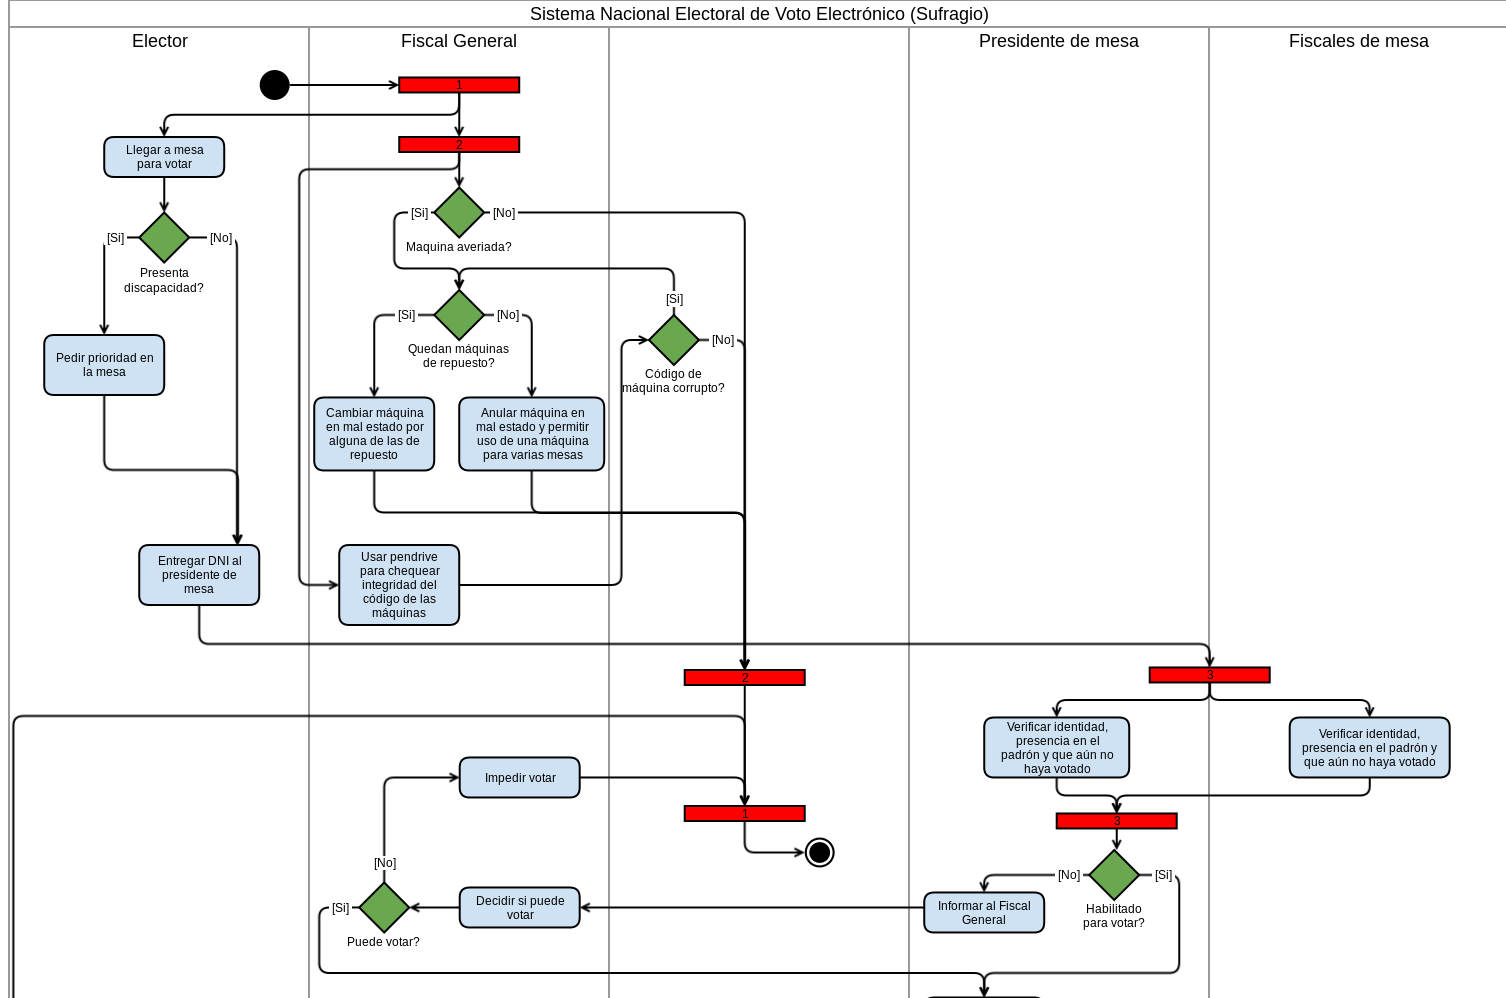
\includegraphics[scale=0.5]{imagenes/actividad/actividadSufragio1}
%\captionof{figure}{Diagrama de actividad}
\end{figure}

\begin{figure}[h!]
\centering
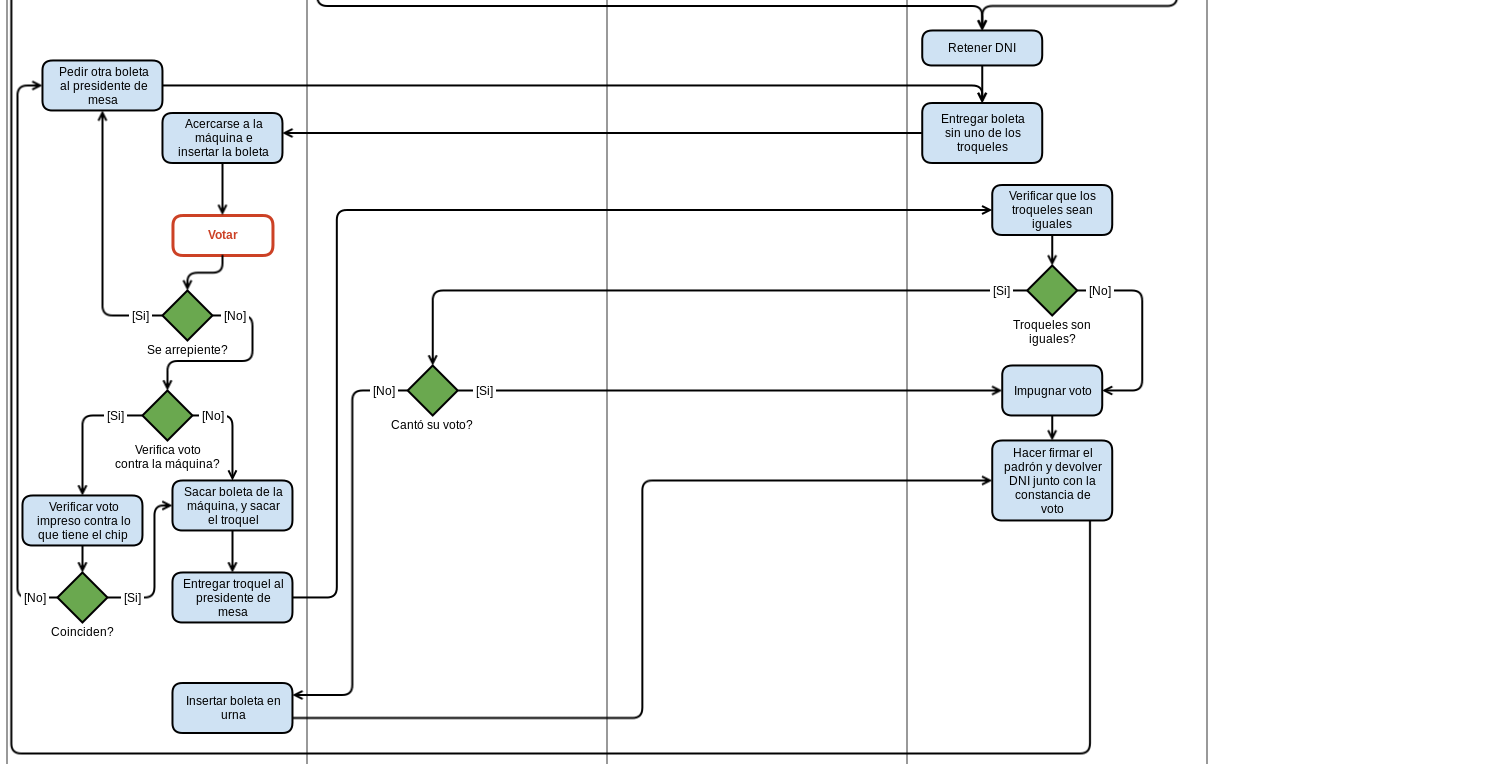
\includegraphics[scale=0.5]{imagenes/actividad/actividadSufragio2}
\end{figure}


\begin{figure}[H]
\centering
%\includegraphics[scale=0.45]{}
%\captionof{figure}{Diagrama de actividad}
\end{figure}
\todo[inline]{Aca va el diagrama de actividad (ojo ocn la escala)}


\subsubsection{Casos de uso}


\textbf{Caso de Uso: }

\textbf{Actores:} 

\textbf{Pre:} 

\textbf{Post:}
\begin{table}[h!]
	
 \begin{tabular}{|p{7.5cm} | p{7.5cm}|} 
 \hline
 \textbf{Curso normal} & \textbf{Curso Alternativo} \\
 \hline

 \end{tabular}

\end{table}


\subsubsection{OCL}

\subsection{Conteo}

\subsubsection{Máquina de estado finito}

\subsubsection{Diagrama de actividad}
\todo[inline]{PONER EN SU LUGAR LOS DIAGRAMAS DE ACTIVIDAD}
\begin{figure}[h!]
\centering
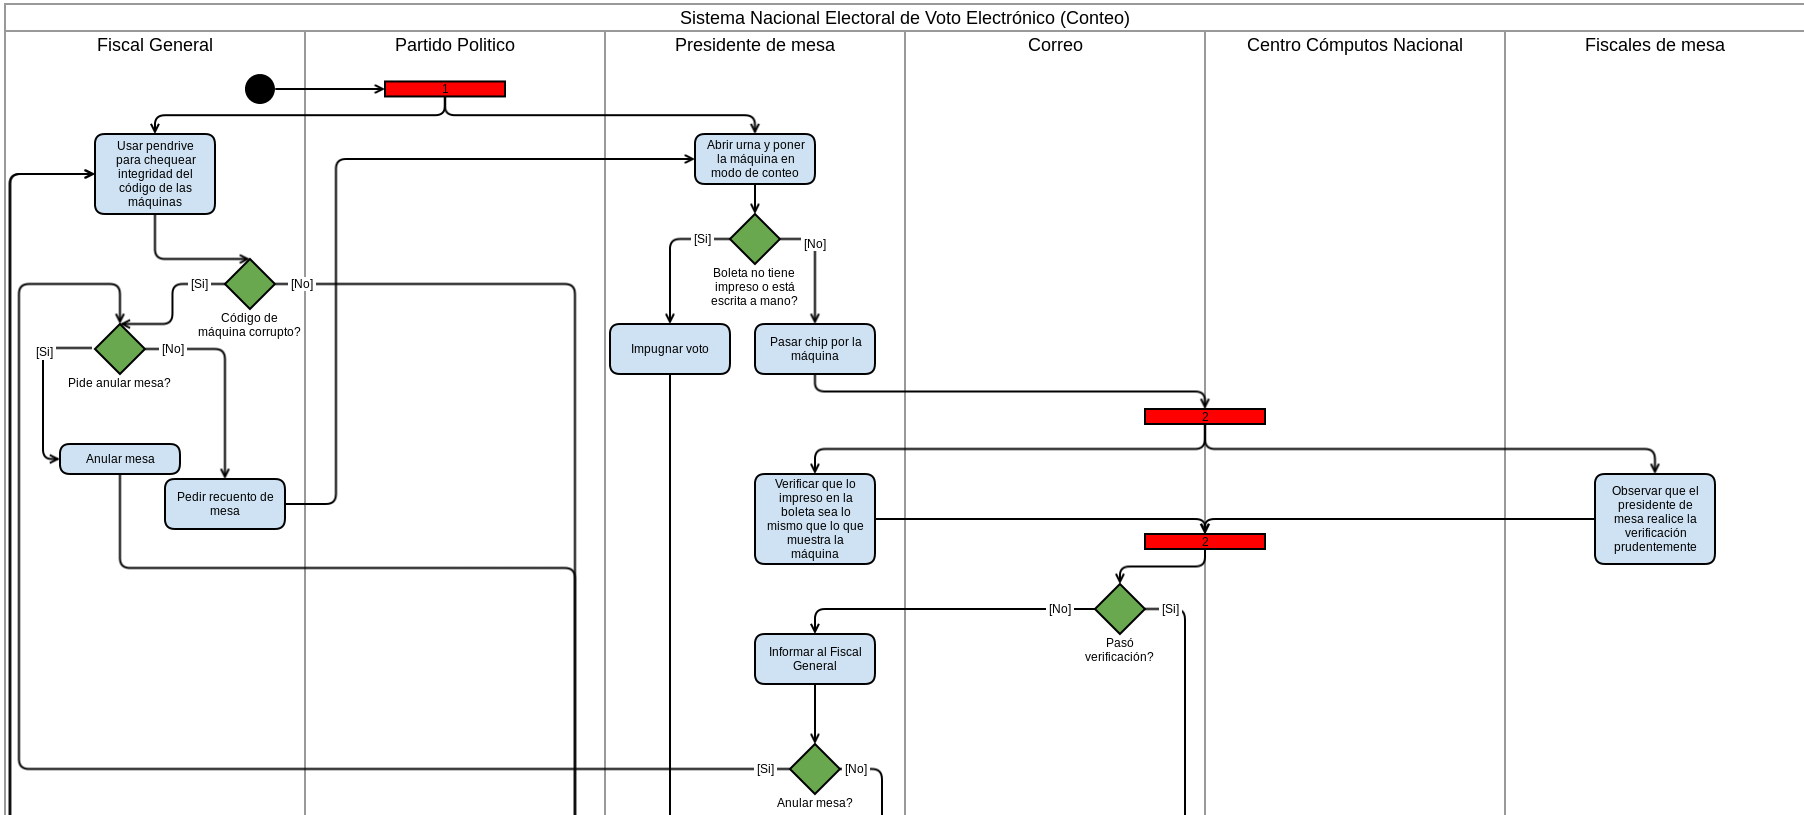
\includegraphics[scale=0.5]{imagenes/actividad/actividadConteo1}
%\captionof{figure}{Diagrama de actividad}
\end{figure}

\begin{figure}[h!]
\centering
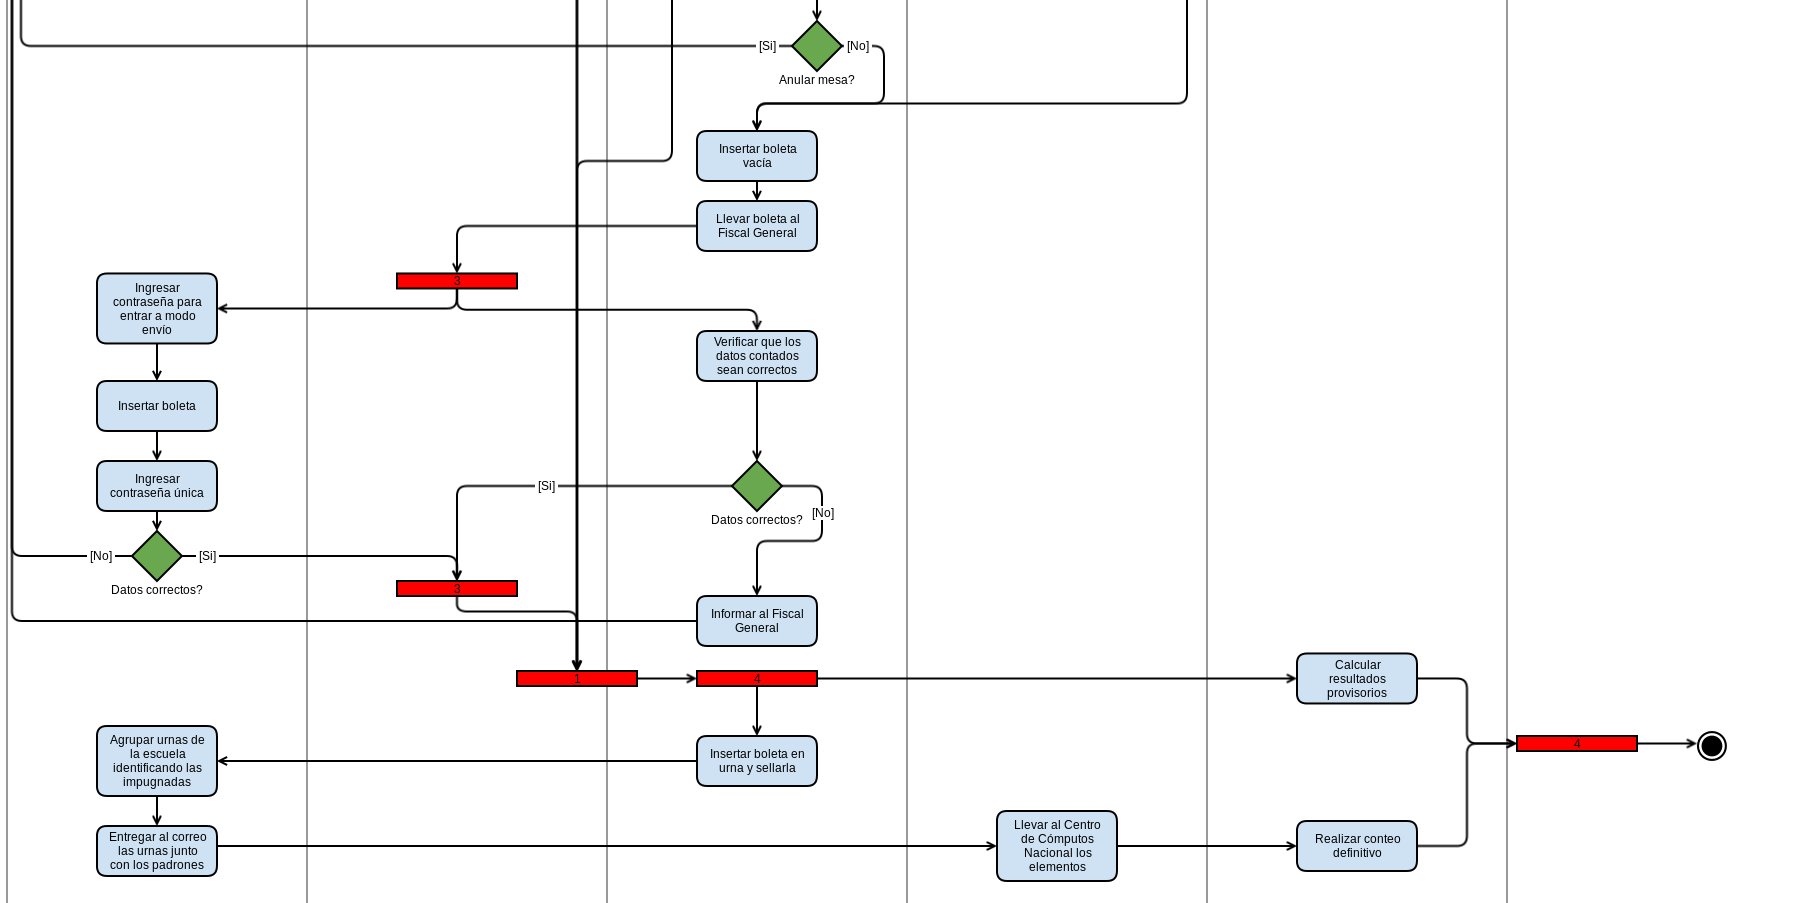
\includegraphics[scale=0.5]{imagenes/actividad/actividadConteo2}
\end{figure}


\begin{figure}[H]
\centering
%\includegraphics[scale=0.45]{}
%\captionof{figure}{Diagrama de actividad}
\end{figure}
\todo[inline]{Aca va el diagrama de actividad (ojo ocn la escala)}

\subsubsection{Casos de uso}


\textbf{Caso de Uso: }

\textbf{Actores:} 

\textbf{Pre:} 

\textbf{Post:}
\begin{table}[h!]
	
 \begin{tabular}{|p{7.5cm} | p{7.5cm}|} 
 \hline
 \textbf{Curso normal} & \textbf{Curso Alternativo} \\
 \hline

 \end{tabular}

\end{table}


\subsubsection{OCL}
\newpage
\section{Discusi\'on}
- Discusión: debe contener un análisis general de lo que los llevó a elegir una técnica respecto a otra. NO DEBE SER una lista de lo que ya se puede desprender del diagrama. Esta sección también es ideal para que vuelquen las cosas que puedan haberles quedado "flojas" o no cerradas del todo: por ejemplo, los aspectos que podrían hacer que todo el sistema no funcione como desean, etc.

Presentaremos a continuación distintos criterios que si bien fueron comentados anteriormente, es importante remarcarlos luego de vistos en partes y algunos puntos que podrian ser evaluados para un futuro análisis

\subsection{Diagrama de actividad vs FSM}

Es fácil ver que estos dos diagramas pueden modelizar muchas cosas equivalentes. Pero cada uno presenta ciertas ventajas frente al otro.
Por ejemplo, a la hora de modelizar un problema con cotas temporales, el diagrama de actividad no es lo suficientemente expresivo. Esto lleva a que las cosas no queden claras y genera confusiones. En cambio el FSM nos permite muy fácilmente gracias al uso de relojes representar cotas temporales en nuestros problemas.

A su vez, las FSM no dan un orden a las acciones, si bien podemos modelar que un actor espera la acción de otro actor para proceder, no es tan expresivo como en el diagrama de actividad donde la acción de cada actor se lleva de manera lineal, vemos perfectamente como es el orden relativo de estas acciones sin necesidad de componer nada, ni de imaginarnos como seria el modelo final de la composición.

Por eso es que utilizamos estos dos diagramas de manera paralela, permite la mejor comprensión del escenario en el que nos encontramos y de los casos de uso.

\subsection{Casos de uso: Refinamiento de acciones}

Podriamos decir que los casos de uso hacen de \textit{refinamiento} de los diagramas antes mencionados. A la hora de implementar este sistema, sera necesario una descripción más profunda de las acciones relacionadas con el sistema, es por eso que utilizamos el diagrama de casos de uso y sus detalles, nos da un panorama bastante preciso sobre cada acción en la interfaz. 

\subsection{Falta de o-refinamientos}

En el trabajo anterior presentamos algunas posibilidades en relación a como lograr algunos objetivos. En este trabajo esa segundas opciones no fueron tomadas en cuenta. Podría haberse estirado el largo de este trabajo haciendo diagramas para estas distintas opciones pero no lo consideramos interesante. 

\subsection{El modelo de clases: Una herramienta descriptiva}

El modelo de clases forma el marco en el cual va a interactuar todo, deja en claro las relaciones entre distintos agentes de nuestro sistema e inserta reglas sobre relaciones. Es sin duda una de los diagramas más importante, si bien no es descriptivo en el sentido temporal. Nos da una visión general de como debe funcionar cada cosa y nos pone junto al diagrama de contexto en una senda sobre los accionares de nuestros actores. 

A su vez, cuantifica las relaciones, sea uno a uno o muchos con muchos de una misma clase, nos queda bien claro que se relaciona con que y nos da un poquito del como, si bien su poder de expresión no sea más que un par de palabras.


\newpage
\section{Conclusiones}
- Conclusiones: mencionar brevemente de qué formas les resultó más sencillo encarar el TP. Por ejemplo en qué orden realizaron los diagramas, qué aspectos presentaron las mayores dificultades, etc.



\end{document}


%\section{Objetivos generales}

%El objetivo de este Trabajo Práctico es ...


%\section{Contexto}

%\begin{figure}
%  \begin{center}
%	
\includegraphics[scale=0.66]{imagenes/logouba.jpg}
%	\caption{Descripcion de la figura}
%	\label{nombreparareferenciar}
%  \end{center}
%\end{figure}


%\paragraph{\textbf{Titulo del parrafo} } Bla bla bla bla.
%Esto se muestra en la figura~\ref{nombreparareferenciar}.

%\begin{codesnippet}
%\begin{verbatim}

%struct Pepe {

%    ...

%};

%\end{verbatim}
%\end{codesnippet}
%\section{Enunciado y solucion} 
%\input{enunciado}
%\section{Conclusiones y trabajo futuro}
